\documentclass[../delivery_hospital_report.tex]{subfiles}
\graphicspath{ {images/}{../images/} }

\begin{document}
\chapter{Distribuição de Energia}

Para o robô hospitalar, levando em consideração que tem uma série de equipamentos sensíveis, como a Jetson Nano \cite{jetson21}, o computador embarcado do projeto, é de extrema importância ter uma fonte de energia estável e segura, para assim, não queimar eventualmente algum equipamento ou lesionar algum dos membros.

Para o projeto todo, somente uma bateria de alta tensão é utilizada e a partir de um regulador de tensão as tensões necessárias para todos os equipamentos é feita.

\section{Bateria DC e Regulador de Tensão}

No geral, como driver do motor usado é feito para um Hoverboard, para facilitar a montagem do robô, utilizamos baterias universais para Hoverboard e partir dela diminuímos a tensão para os demais parelho, como os ESP32 \cite{esp32}, que recebem 12V e a Jetson que recebe 5V.

\begin{figure}[h]
\centering
    \caption{Bateria de Bateria Universal Hoverboard}
    \centering % para centralizarmos a figura
    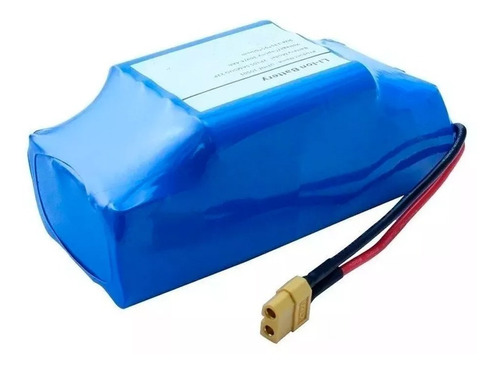
\includegraphics[width=10cm]{baterry_used.jpg}
    \caption*{Fonte: retirado de \cite{drivermotor21}}
    \label{fig:Bateria de Bateria Universal Hoverboard}
\end{figure}

Para diminuir a tensão de 36V baterias universais para Hoverboard, foi utilizado um regulador de tensão chaveado buck \cite{reguladorcha21}, que abaixaria a tensão da bateria para 12V e 5V, que é o suficiente para tanto os meus embarcado, quanto a Jetson Nano.

\end{document}